% !TEX program = lualatex
% !TEX spellcheck = it_IT

% !TEX program = lualatex
% !TEX root = ./relazioni.tex

\documentclass[ structure      = article
              , maketitlestyle = standard
              , secstyle       = center
              , secfont        = roman
              %, subsecstyle    = center
              , subsecfont     = roman
              , headerstyle    = center
              , liststyle      = aligned
              , twocolcontents = toc
              ]{suftesi}

\usepackage[no-math]{fontspec}
\setmainfont{Linux Libertine O}
\setmonofont{Source Code Pro}[Scale=MatchLowercase]
%\usepackage[tt=false]{libertine}
%\usepackage{sourcecodepro}

\usepackage{polyglossia}
\setmainlanguage{italian}
\setotherlanguage{english}

\usepackage[italian=quotes]{csquotes}

\usepackage{hyperref}
\hypersetup{breaklinks,hidelinks}

\usepackage{anyfontsize}

\usepackage{indentfirst}

%\usepackage[original]{abstract}
%\renewcommand{\abstracttextfont}{\normalfont\normalsize}

\usepackage{libertinust1math}
\usepackage{MnSymbol,mathtools}
\usepackage[bb=ams]{mathalfa}
\usepackage{amsthm}
\theoremstyle{definition}
\newtheorem{esercizio}{Esercizio}[section]
\newtheorem{nota}{Nota}[section]

\usepackage{listings,xcolor}
\lstset{
    language        = Matlab
  , basicstyle      = \small\ttfamily
  , commentstyle    = \color{green!50!black}
  , keywordstyle    = \color{blue!50!black}
  %, tabsize         = 2
  , numbers         = left
  , numberstyle     = \tiny\ttfamily\color{gray!50!black}
  , numbersep       = 2mm
  , frame           = leftline
  , rulecolor       = \color{gray!50!black}
  , backgroundcolor = \color{gray!3!white}
  %, mathescape      = true
  }


\newcommand\set[1]{\left\{#1\right\}}
\newcommand\abs[1]{\left\lVert #1 \right\rVert}
\newcommand\erre{\mathbb R}
\newcommand\enne{\mathbb N}


\title{Analisi Numerica \\ Relazioni di Laboratorio}
\author{Indrjo Dedej}
\date{Ultima revisione: \today{}.}

\begin{document}

\maketitle

\tableofcontents

\begin{nota}
Per la parte dei codici è stato usato {\tt GNU Octave} al posto di {\tt Matlab}.
\end{nota}

\begin{nota}
Se \(A\) è il nome di una matrice, allora scriviamo \(A_{i,j}\) per indicare l'entrata di \(A\) alla \(i\)-esima riga e \(j\)-esima colonna.
\end{nota}

% !TEX program = lualatex
% !TEX root = ../relazioni.tex
% !TEX spellcheck = it_IT

\section{Metodi diretti per sistemi lineari}

\begin{esercizio}
Scrivere una funzione \lstinline£tri_solve£ che prenda in input una matrice triangolare \(A\) e un vettore \(b\) e calcoli la soluzione del sistema lineare \(Ax = b\). Tale funzione deve gestire sia il caso triangolare superiore che triangolare inferiore (si usino eventualmente le funzioni \lstinline£istriu£ e \lstinline£istril£).
\end{esercizio}

Una matrice quadrata \(A\) di ordine \(n\) si dice {\em triangolare superiore} (rispettivamente, {\em inferiore}) qualora \(A_{i, j} = 0\) per ogni \(i, j \in \set{1, \dots{}, n}\) con \(i > j\) (rispettivamente, \(i < j\)). Un sistema triangolare inferiore è quindi fatto quindi di equazioni
\[\sum_{j = 1}^i A_{i, j} x_j = b_i \quad\text{per } i \in \set{1, \dots{}, n} .\]
Si verifica immediatamente che la soluzione \(x := \begin{bmatrix} x_1 & \cdots{} & x_n \end{bmatrix}^T\) di questo sistema è tale che
\begin{align*}
& x_1 = \frac{b_1}{A_{1,1}} \\
& x_i = \frac{1}{A_{i, i}} \left(b_i -\sum_{j = 1}^{i-1} A_{i, j} x_j\right)
\end{align*}

La funzione qui sotto prende una matrice triangolare inferiore \(A\) e un vettore \(b\) e restituisce la soluzione del sistema \(Ax = b\).

\lstinputlisting{../metodi-diretti/solve\_lower\_triangular.m}

Invece, la soluzione \(x := \begin{bmatrix} x_1 & \cdots{} & x_n \end{bmatrix}^T\) di un sistema triangolare superiore
\[\sum_{j = n-i+1}^{n} A_{i, j} x_j = b_i \quad\text{per } i \in \set{1, \dots{}, n}\]
è data da
\begin{align*}
& x_n = \frac{b_n}{A_{n,n}} \\
& x_{n-i+1} = \frac{1}{A_{n-i+1, n-i+1}} \left(b_n -\sum_{j = n-i+2}^{i-1} A_{i, j} x_j\right)
\end{align*}

La funzione che risolve \(Ax = b\) nel caso in cui \(A\) sia triangolare superiore è:

\lstinputlisting{../metodi-diretti/solve\_upper\_triangular.m}

Pertanto la funzione che risolve un sistema triangolare \(Ax = b\) è la seguente.

\lstinputlisting{../metodi-diretti/solve\_triangular.m}


\begin{esercizio}
Scrivere due funzioni, \lstinline£lu_nopiv£ e \lstinline£lu_piv£, che calcolino la fattorizzazione LU con e senza pivoting di una matrice, rispettivamente.
\end{esercizio}

L'algoritmo di eliminazione gaussiana consente, presa una matrice invertibile \(A\) di ordine \(n\), di trasformare il sistema
\[A x = b\]
in uno equivalente
\[U x = b'\]
dove \(U\) è triangolare superiore. Il passaggio da \(A\) ad \(U\) avviene attraverso una matrice \(L\) triangolare inferiore con gli elementi sulla diagonale principale uguali ad \(1\):
\[A = LU .\]
Le entrate della matrice \(L\) sono ottenute durante l'algoritmo di Gauss. Qui sotto ci sono le funzioni che ad una matrice \(A\) restituisce la fattorizzazione LU, la prima senza e la seconda con pivotazione. 

\lstinputlisting{../metodi-diretti/lu\_nopiv.m}

La fattorizzazione LU con pivotazione coinvolge un'altra matrice:
\[PA = LU\]
dove \(P\) è ottenuta dall'identità permutandone le righe.

\lstinputlisting{../metodi-diretti/lu\_piv.m}

\begin{esercizio}
Scrivere una funzione che, presa in input una matrice reale \(A\) di ordine \(n\) non singolare, ne calcoli l'inversa usando la fattorizzazione LU.
\end{esercizio}

In generale, l'inversa di \(A\) è una matrice \(X = \begin{bmatrix} x_1 & \cdots{} & x_n\end{bmatrix}\) tale che
\[A x_i = e_i \quad\text{per } i \in \set{1, \dots{}, n} .\]
Si tratta quindi di risolvere \(n\) sistemi lineari. Quando è disponibile la fattorizzazione LU di \(A\), però si può seguire una strada che usa quanto implementato prima, ma che aumenta il numero di sistemi da risolvere. Sia quindi \(PA = LU\), e quindi i sistemi diventano
\[LU x_i = P e_i .\]

Le soluzioni \(x_i\) si determinano risolvendo i sistemi triangolari
\[Ly_i = Pe_i \quad\text{e}\quad Ux_i = y_i \quad\text{per } i \in \set{1, \dots{}, n} .\]

\lstinputlisting{../metodi-diretti/inverse\_lu.m}

\begin{esercizio}
Scrivere una funzione che calcola il determinante di una matrice \(A\) usando la fattorizzazione \(PA = LU\). Per calcolare il determinate di \(P\), si modifichi la funzione scritta al punto 2 in modo da contare il numero di scambi di righe effettuati.
\end{esercizio}

Da \(PA = LU\) abbiamo che \(\det P \det A = \det L \det U = \det U\). Essendo \(P\) una permutazione delle righe dell'identità, si ha \(\det P = \pm 1\). Inoltre si nota che \(P P = I\). Quindi, in principio, la funzione qui sotto potrebbe andare bene.

\lstinputlisting{../metodi-diretti/lu\_det1.m}

Tuttavia questa implementazione richiede inutilmente alla macchina di calcolare \(L\). Inoltre di \(P\) si sa che è \(I\) con le righe permutate, quindi \(\det P\) è \(1\) se c'è stato un numero pari di scambi, \(-1\) altrimenti. In breve, \(\det P = (-1)^\delta\), dove \(\delta\) è il numero di scambi di righe effettuati. Una versione più economica quindi è:

\lstinputlisting{../metodi-diretti/lu\_det2.m}


\begin{esercizio}
Scrivere due funzioni \lstinline£sgs£ e \lstinline£mgs£ che calcolino la fattorizzazione QR ridotta di una matrice, usando rispettivamente il metodo di Gram-Schmidt e il metodo di Gram-Schmidt modificato.
\end{esercizio}

Siano \(a_1, \dots{}, a_n \in \erre^m\) linearmente indipendenti. L'{\em algoritmo di Gram-Schmidt} dà \(n\) vettori \(q_1, \dots{}, q_n \in \erre^m\) tra loro ortogonali:
\begin{align*}
q_1 & := x_1 \\
q_i & := x_i - \sum_{j=1}^{i-1} \frac{q_j^T x_i}{\abs{q_j}^2} q_j = x_i - \sum_{j=1}^{i-1} \left[\left(\frac{q_j}{\abs{q_j}}\right)^T x_i \right] \frac{q_j}{\abs{q_j}} \quad\text{per } i \in \set{2, \dots{}, n}
\end{align*}
%
%Si possono ottenere anche una \(n\)-upla di vettori ortonormali \(\hat q_1, \dots{}, \hat q_n \in R^m\) dove \(\hat q_i := \frac{q_i}{\abs {q_i}}\).
%
Se introduciamo la matrice \(R\) triangolare superiore attraverso
\[R_{j,i} := \begin{cases} \abs{q_i} & \text{se } i= j \\ \left(\frac{q_j}{\abs{q_j}}\right)^T x_i & \text{se } j \le i-1 \\ 0 & \text{altrimenti} \end{cases}\]
possiamo scrivere
\[X = Q R ,\]
dove \(Q := \begin{bmatrix} \frac{q_1}{\abs {q_1}} & \cdots{} & \frac{q_n}{\abs {q_n}} \end{bmatrix}\).

Ecco l'implementazione di questo algoritmo.

\lstinputlisting{../metodi-diretti/sgs.m}

Per ragioni numeriche, è meglio però l'implementazione che segue:

\lstinputlisting{../metodi-diretti/mgs.m}


\begin{esercizio}
Sia \(m = 50\) e \(n = 12\). Sia \(f(t) = \cos(4t)\) e si definiscano i punti \(t_i = \frac{i-1}{m-1}\) per \(i = 1, \dots{}, m\) e \(b\) il vettore di componenti \(b_i = f(t_i)\). Sia \(A\) la matrice del problema dei minimi quadrati che si ottiene approssimando con un polinomio di grado \(n-1\) la sequenza dei punti \((t_i, b_i)\). Si risolva e visualizzi (con tutti e sedici i decimali) la soluzione del problema calcolata con i seguenti metodi:
\begin{enumerate}
\item formazione e soluzione del sistema di equazioni normali usando il comando \lstinline£\£ di MATLAB
\item fattorizzazione QR utilizzando \lstinline£sgs£
\item fattorizzazione QR utilizzando \lstinline£mgs£
\item fattorizzazione QR utilizzando \lstinline£qr£ (funzione built-in di MATLAB che utilizza il metodo di Householder).
\end{enumerate}
I calcoli precedenti generano quattro liste di 12 coefficienti. Prendendo come riferimento la soluzione con l'ultimo metodo, si cancellino in ogni lista le cifre decimali che appaiono errate (affette da arrori di arrotondamento). Quali metodi si mostrano più instabili? Non è necessario spiegare le osservazioni fatte.
\end{esercizio}

In generale, presi \(m\) punti \((x_1, y_1)\), \dots{} e \((x_m, y_m)\) di \(\erre^2\), si cerca un polinomio \(p_\ast \in \mathbb P_n\), con \(n < m-1\), tale che
\[\sum_{i = 1}^m (p_\ast(x_i) - y_i)^2 \le \sum_{i = 1}^m (p(x_i) - y_i)^2 \quad \text{per ogni } p \in \mathbb P_n .\]
Per ricondurci al problema dei minimi quadrati, basta osservare che, se
\[p(x) = c_1 + c_2 x + c_3 x^3 + \dots{} + c_{n+1} x^n \,\]
allora
\[\sum_{i = 1}^m (p(x_i) - y_i)^2 = \lVert A c - y \rVert_2^2\]
dove
\[A := \begin{bmatrix}
1 & x_1 & x_1^2 & \cdots{} & x_1^n \\
\vdots{} & \vdots{} & \vdots{} & \vdots{} & \vdots{} \\
1 & x_i & x_i^2 & \cdots{} & x_i^n \\
\vdots{} & \vdots{} & \vdots{} & \vdots{} & \vdots{} \\
1 & x_m & x_m^2 & \cdots{} & x_m^n\end{bmatrix} \in \erre^{m \times (n+1)} .\]
Per trovare quindi il \(p_\ast \in \mathbb P_n\) che minimizza \(\sum_{i = 0}^n (p(x_i) - y_i)^2\) è equivalente a trovare il \(c \in \erre^{n+1}\) che minimizza \(\lVert Ac -y \rVert_2^2\). Cioè si deve risolvere l'equazione
\[A^T A c = A^T y\]
rispetto a \(c\).

Diamo una funzione che presa una lista di ascisse \(x \in \erre^m\) e un numero naturale \(n\) produce la matrice \(A\) di sopra:

\lstinputlisting{../metodi-diretti/vandermonde.m}

Diamo a anche le seguenti funzioni che risolvono il problema nei modi richiesti nell'ordine.

\lstinputlisting{../metodi-diretti/minquad.m}

Se usiamo la decomposizione \(A = Q R\) dell'esercizio precedente, allora
\[R^T \underbrace{Q^T Q}_{= I} R c = R^T Q^T y\]
da cui, perché \(R\) è triangolare,
\[R c = Q^T y .\]
Le funzioni che seguono si basano sulla risoluzione di questa equazione. Abbiamo già dato negli esercizi precedenti le funzioni che risolvono sistemi triangolari superiori.

\lstinputlisting{../metodi-diretti/minquad\_sgs.m}
\lstinputlisting{../metodi-diretti/minquad\_mgs.m}
\lstinputlisting{../metodi-diretti/minquad\_qr.m}

Testiamo le funzioni appena implementate. Prima di tutto, diamo i vettori di \(\erre^{50}\):
\begin{lstlisting}[numbers=none]
octave> format long
octave> t = (@(i) (i-1)/49)(1:50)';
octave> b = (@(x) cos(4*x))(t);
\end{lstlisting}

Chiediamo ora di risolvere il problema ai minimi quadrati, usando un polinomi di grado \(11\):

%\noindent
%\begin{minipage}{.45\textwidth}
\begin{lstlisting}[numbers=none]
octave> c1 = minquad(11, t, b)
c1 =

   9.999999998598327e-01
  -1.637969801790591e-07
  -7.999989743148679e+00
  -2.072197377938371e-04
   1.066866439686697e+01
  -1.069780529188339e-02
  -5.655104676152303e+00
  -6.193169964808305e-02
   1.679168741518508e+00
   1.575953725551536e-02
  -3.779623750302716e-01
   8.865738750316085e-02
\end{lstlisting}
%\end{minipage}
%
%\hfill
%
%\begin{minipage}{.45\textwidth}
\begin{lstlisting}[numbers=none]
octave> c2 = minquad_sgs(11, t, b)
c2 =

   1.000010858217736e+00
  -1.597441622479323e-03
  -7.961790735605575e+00
  -3.563609846100917e-01
   1.232237295279629e+01
  -4.198742022992519e+00
   1.143539843615144e-01
  -3.712350976158632e+00
   1.556815307967554e+00
   1.317363348240178e+00
  -7.841381000343972e-01
   5.040691898039995e-02
\end{lstlisting}
%\end{minipage}

%\noindent
%\begin{minipage}{.45\textwidth}
\begin{lstlisting}[numbers=none]
octave> c3 = minquad_mgs(11, t, b)
c3 =

   9.999999993467416e-01
   2.936344856152573e-08
  -7.999997687339061e+00
  -8.218757375288988e-05
   1.066765586643305e+01
  -5.947011668467894e-03
  -5.669068083108868e+00
  -3.556294157169759e-02
   1.647176449303515e+00
   3.985971841029823e-02
  -3.882198705396149e-01
   9.054209982423345e-02
\end{lstlisting}
%\end{minipage}
%
%\hfill
%
%\begin{minipage}{.45\textwidth}
\begin{lstlisting}[numbers=none]
octave> c4 = minquad_qr(11, t, b)
c4 =

   1.000000000996612e+00
  -4.227432497394545e-07
  -7.999981235680764e+00
  -3.187632846675115e-04
   1.066943079626799e+01
  -1.382028918305878e-02
  -5.647075624787249e+00
  -7.531602913513780e-02
   1.693606968736276e+00
   6.032105768099427e-03
  -3.742417020548601e-01
   8.804057586530689e-02
\end{lstlisting}
%\end{minipage}


% !TEX program = lualatex
% !TEX root = ../relazioni.tex
% !TEX spellcheck = it_IT

\section{Metodi di ricerca di zeri}

\begin{figure}
\centering
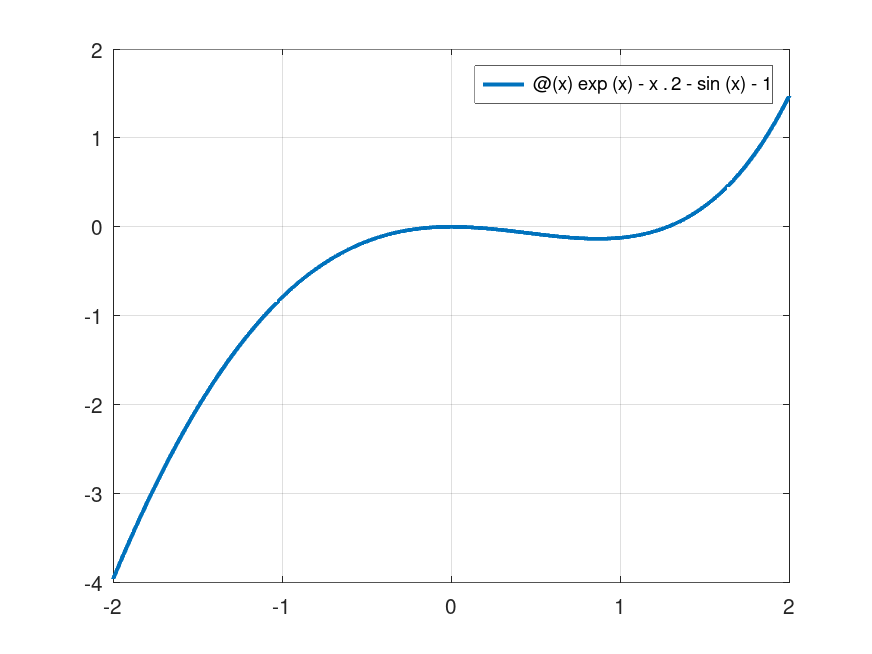
\includegraphics[width=.7\textwidth]{../zeri/graph1.png}
\caption{Grafico di \(f(x) := e^x - x^2 - \sin x - 1\)}
\end{figure}

\begin{esercizio}
Scrivere una funzione
\begin{center}
\lstinline£[c, fc, iter] = bisezione(f, a, b, tol, itmax)£
\end{center}
metodo di bisezione per la ricerca di una funzione \lstinline£f£ nell'intervallo \lstinline£[a, b]£. Qui, \lstinline£tol£ è la tolleranza sull'approssimazione della radice e \lstinline£itmax£ è il numero massimo di iterazioni disposte a fare. Per quanto riguarda l'output, \lstinline£c£ è l'approssimazione trovata, \lstinline£fc£ è \lstinline£f(c)£ e \lstinline£iter£ è il numero di iterazioni fatte effettivamente per arrivare all'approssimazione \lstinline£c£. Testare la funzione per la ricerca di una delle radici di
\[f(x) := e^x - x^2 - \sin x - 1\]
sull'intervallo \([-2, 2]\).
\end{esercizio}

L'implementazione qui sotto usa il {\em teorema degli zeri}\footnote{Sia \(f : [a, b] \to \erre\) continua con \(f(a)f(b) < 0\). Allora esiste \(c \in ]a, b[\) tale che \(f(c) = 0\).} e l'algoritmo di bisezione che descriviamo velocemente.
\begin{enumerate}
\item Iniziamo con \([a_0, b_0] := [a, b]\).
\item Per \(n \in \enne\), consideriamo \([a_n, b_n]\). Se \(f\) si annulla in uno tra i punti \(a_n, b_n, c_n := \frac{a_n+b_n}{2}\), allora qualche zero è stato individuato. Altrimenti, si dà l'intervallo
\[[a_{n+1}, b_{n+1}] := \begin{cases} [a_n, c_n] & \text{se } f(a_n)f(c_n) < 0 \\ [c_n, b_n] & \text{se } f(c_n)f(b_n) > 0 \end{cases}.\]
\end{enumerate}
A tal scopo è utile osservare che per ogni \(c \in [a_n, b_n]\) si ha
\[\lvert c-c_n \rvert \le \frac{b_n - a_n}{2} = \frac{b_0 - a_0}{2^{n+1}} \text{ per ogni } n \in \enne .\]
Questa disuguaglianza dà un stima dell'errore commesso al passo \(n\)-esimo. Ovviamente, per un'implementazione al calcolatore non possiamo procedere indefinitamente: scegliamo di arrestarci quando viene superato un certo limite di iterazioni oppure quando il numero \(\frac{b_n - a_n}{2}\) scende sotto un valore fissato.

\lstinputlisting{../zeri/bisezione.m}

Testiamo il metodo di bisezione su \(f\):

\begin{lstlisting}[numbers=none]
octave> f = @(x) exp(x)-x.^2-sin(x)-1;
octave> [c, fc, iter] = bisezione(f, 1, 1.5, 1e-12, 100)
c = 1.279701331001888
fc = 6.681322162194192e-13
iter = 39
\end{lstlisting}

% *********************************************************************************************

\begin{esercizio}
Scrivere una funzione
\begin{center}
\lstinline£[c, fc, iter] = newton(f, df, x0, tol, itmax)£
\end{center}
che implementa il metodo di \textenglish{Newton-Raphson} per la ricerca di uno zero di una funzione \lstinline£f£ con derivata \lstinline£df£. Qui, \lstinline£x0£ è il punto da cui parte il metodo, \lstinline£tol£ è la tolleranza sull'approssimazione della radice e \lstinline£itmax£ è il numero massimo di iterazioni disposte a fare. Per quanto riguarda l'output, \lstinline£c£ è l'approssimazione trovata, \lstinline£fc£ è \lstinline£f(c)£ e \lstinline£iter£ è il numero di iterazioni fatte effettivamente per arrivare all'approssimazione \lstinline£c£. Testare la funzione per la ricerca di una delle radici di
\[f(x) := e^x - x^2 - \sin x - 1\]
sull'intervallo \([-2, 2]\).
\end{esercizio}

Richiamiamo che il metodo di \textenglish{Newton-Raphson} si scrive come
\[\begin{cases} x_0 \in \erre \text{ scelto} \\ x_{n+1} = x_n - \frac{f(x_n)}{f^\prime (x_n)} \text{ per } n \in \enne \end{cases}\]

Osserviamo che se dobbiamo controllare l'incremento, ci dobbiamo arrestare quando il valore assoluto di \(\frac{f(x_n)}{f^\prime (x_n)}\) scende al di sotto di una certa tolleranza. Anche in questo caso imponiamo un numero massimo di iterazioni. 

\lstinputlisting{../zeri/newton.m}

Testiamo questo metodo su \(f\):

\begin{lstlisting}[numbers=none]
octave> f = @(x) exp(x)-x.^2-sin(x)-1;
octave> df = @(x) exp(x)-2*x-cos(x);
octave> [c, fc, iter] = newton(f, df, 2, 1e-6, 100)
c = 1.279701331001091
fc = 7.083222897108499e-14
iter = 6
\end{lstlisting}

% *********************************************************************************************

\begin{figure}
\centering
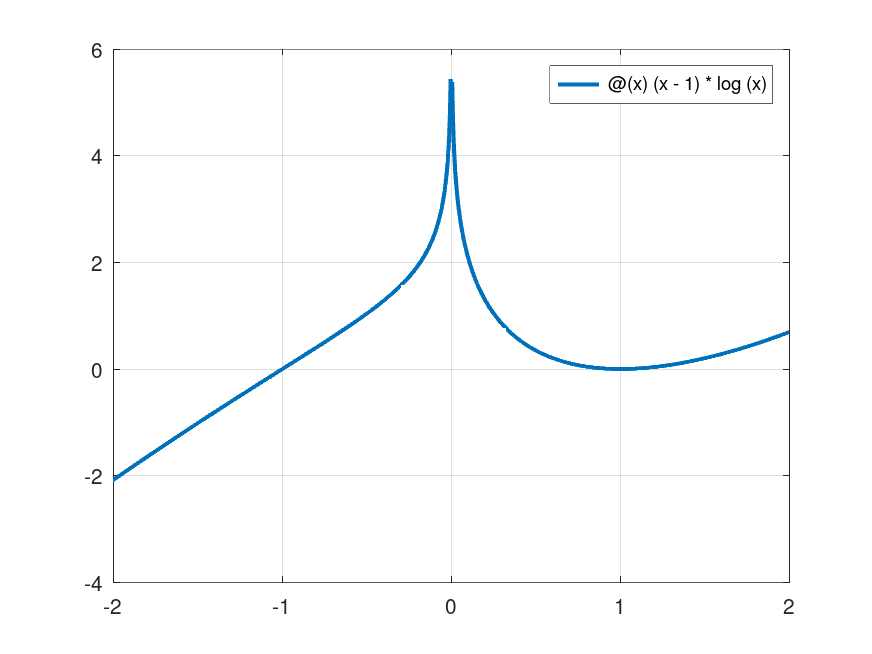
\includegraphics[width=.7\textwidth]{../zeri/graph2.png}
\caption{Grafico di \(f(x) = (x-1)\ln x\)}
\end{figure}

\begin{figure}
\centering
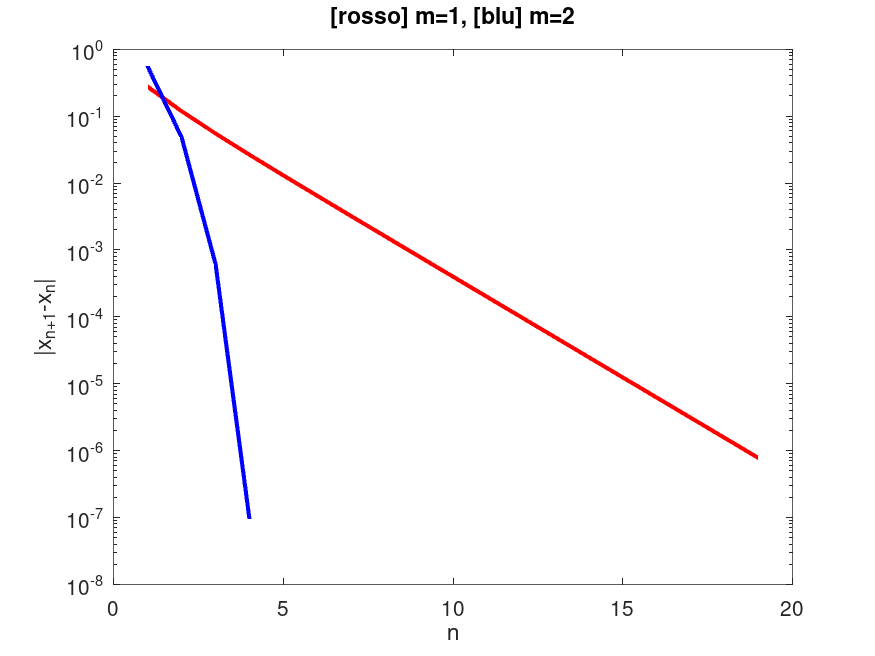
\includegraphics[width=.7\textwidth]{../zeri/convergences.png}
\caption{Grafico degli incrementi al variare del numero di iterazioni}
\label{fig:convergences}
\end{figure}

\begin{esercizio}
Considerare la funzione \(f(x) = (x-1)\ln x\). Applicare il metodo di \textenglish{Newton-Raphson} e il metodo di \textenglish{Newton-Raphson} {\em modificato} per la ricerca della radice doppia \(1\) e confrontare graficamente gli ordini di convergenza dei due metodi.
\end{esercizio}

Se \(\alpha\) è una radice con molteplicità \(m \ge 2\), il metodo di \textenglish{Newton-Raphson} ha ordine \(1\). Se però sappiamo a priori \(m\), possiamo modificare questo metodo così:
\[\begin{cases} x_0 \in \erre \text{ scelto} \\ x_{n+1} = x_n - m\frac{f(x_n)}{f^\prime (x_n)} \text{ per } n \in \enne \end{cases}\]
ed avere una convergenza quadratica.

Modifichiamo \lstinline£newton£ in questo modo: tra gli output teniamo conto di \(m\), c'è un solo output questa volta ed è una lista degli incrementi \(\left\lvert x_{n+1} - x_n \right\rvert\).

\lstinputlisting{../zeri/newton\_errors.m}

Il seguente script disegna il grafico che permette di confrontare la velocità di convergenza nei casi \lstinline£m=1£ e \lstinline£m=2£.

\lstinputlisting{../zeri/convergences.m}


\end{document}
